\documentclass[12pt]{article}
\usepackage[utf8]{inputenc}
\usepackage{geometry}
\geometry{letterpaper, margin=0.25in}
\usepackage{graphicx} 
\usepackage{parskip}
\usepackage{booktabs}
\usepackage{array} 
\usepackage{paralist} 
\usepackage{verbatim}
\usepackage{subfig}
\usepackage{fancyhdr}
\usepackage{sectsty}
\usepackage[shortlabels]{enumitem}

\pagestyle{fancy}
\renewcommand{\headrulewidth}{0pt} 
\lhead{}\chead{}\rhead{}
\lfoot{}\cfoot{\thepage}\rfoot{}

%%% ToC (table of contents) APPEARANCE
\usepackage[nottoc,notlof,notlot]{tocbibind} 
\usepackage[titles,subfigure]{tocloft}
\renewcommand{\cftsecfont}{\rmfamily\mdseries\upshape}
\renewcommand{\cftsecpagefont}{\rmfamily\mdseries\upshape} %

\usepackage{amsmath}
\usepackage{amssymb}
\usepackage{mathtools}
\usepackage{empheq}
\usepackage{xcolor}
\usepackage{bbm}
\usepackage{tikz}
\usepackage{pgfplots}
\usepackage{tikz-cd}
\pgfplotsset{compat=1.18}
\usetikzlibrary{intersections, decorations.markings}
\tikzset{
    marking along/.style n args={2}{
        decoration={
                markings, 
                mark=at position #1 with {\arrow{#2}}
        },
        postaction={decorate}
        },
    marking along/.default={0.5}{>}
}

\newcommand{\ans}[1]{\boxed{\text{#1}}}
\newcommand{\vecs}[1]{\langle #1\rangle}
\renewcommand{\hat}[1]{\widehat{#1}}

\renewcommand{\P}{\mathbb{P}}
\newcommand{\R}{\mathbb{R}}
\newcommand{\E}{\mathbb{E}}
\newcommand{\Z}{\mathbb{Z}}
\newcommand{\N}{\mathbb{N}}
\newcommand{\Q}{\mathbb{Q}}
\newcommand{\C}{\mathbb{C}}

\newcommand{\ind}{\mathbbm{1}}
\newcommand{\qed}{\quad \blacksquare}

\newcommand{\brak}[1]{\left\langle #1 \right\rangle}
\newcommand{\bra}[1]{\left\langle #1 \right\vert}
\newcommand{\ket}[1]{\left\vert #1 \right\rangle}

\newcommand{\abs}[1]{\left\vert #1 \right\vert}
\newcommand{\mfX}{\mathfrak{X}}
\newcommand{\ep}{\varepsilon}

\newcommand{\Ec}{\mathcal{E}}
\newcommand{\A}{\mathcal{A}}
\newcommand{\F}{\mathcal{F}}
\newcommand{\Cc}{\mathcal{C}}
\newcommand{\B}{\mathcal{B}}
\newcommand{\M}{\mathcal{M}}
\newcommand{\X}{\chi}
\renewcommand{\L}{\mathcal{L}}

\newcommand{\sub}{\subseteq}
\newcommand{\st}{\text{ s.t. }}
\newcommand{\card}{\text{card }}
\renewcommand{\div}{\vspace*{10pt}\hrule\vspace*{10pt}}
\newcommand{\surj}{\twoheadrightarrow}
\newcommand{\inj}{\hookrightarrow}
\newcommand{\biject}{\hookrightarrow \hspace{-8pt} \rightarrow}
\renewcommand{\bar}[1]{\overline{#1}}
\newcommand{\overcirc}[1]{\overset{\circ}{#1}}
\newcommand{\diam}{\text{diam }}

\renewcommand{\Re}{\text{Re}\,}
\renewcommand{\Im}{\text{Im}\,}
\newcommand{\sign}{\text{sign}\,}

\newcommand*{\tbf}[1]{\ifmmode\mathbf{#1}\else\textbf{#1}\fi}

\usepackage{tcolorbox}
\tcbuselibrary{breakable, skins}
\tcbset{enhanced}
\newenvironment*{tbox}[2][gray]{
    \begin{tcolorbox}[
        parbox=false,
        colback=#1!5!white,
        colframe=#1!75!black,
        breakable,
        title={#2}
    ]}
    {\end{tcolorbox}}

\newenvironment*{exercise}[1][red]{
    \begin{tcolorbox}[
        parbox=false,
        colback=#1!5!white,
        colframe=#1!75!black,
        breakable
    ]}
    {\end{tcolorbox}}

\newenvironment*{proof}[1][blue]{
\begin{tcolorbox}[
    parbox=false,
    colback=#1!5!white,
    colframe=#1!75!black,
    breakable
]}
{\end{tcolorbox}}

\title{APMA 1360: Homework 4}
\author{Milan Capoor}
\date{21 February 2025}

\begin{document}
\maketitle
\section{Stability of linear systems}

Consider a linear system of the form $\dot{u}=Au$, where $A$ is a real $n\times n$ matrix with eigenvalues $\lambda_1,\ldots,\lambda_n\in\mathbb{C}$. We classify the equilibrium $u=0$ as\\
\hspace*{1in}\begin{tabular}{ll}
    attractor     & if $\Re\lambda_j<0$ for all $j$,                                                                       \\
    repeller      & if $\Re\lambda_j>0$ for all $j$,                                                                       \\
    saddle        & if $\Re\lambda_j\neq0$ for all $j$, and there are two indices $i,k$ with $\Re\lambda_i<0<\Re\lambda_k$ \\
    nonhyperbolic & if $\Re\lambda_j=0$ for at least one index $j$.
\end{tabular}

\begin{enumerate}[(i)]
    \item Argue that these four cases exhaust all possibilities and sketch three sample phase diagrams for planar systems where $u=0$ is, respectively, an attractor, repeller, or saddle (you can choose $A$ to be a diagonal matrix for these examples).

          \color{blue}
          Suppose $n =1$, i.e. the only eigenvalue is $\lambda_1$. In this case, we must have $\Re\lambda_1 < 0$, $\Re \lambda_1 > 0$, or $\Re \lambda_1 = 0$. All cases are covered by the above classification.

          Now take $n=2$, WLOG $\lambda_1, \lambda_2$. We have the following possible cases by sheer enumeration:
          \begin{itemize}
              \item $\Re \lambda_1 < 0$ and $\Re \lambda_2 < 0$: Attractor
              \item $\Re \lambda_1 > 0$ and $\Re \lambda_2 > 0$: Repeller
              \item $\Re \lambda_1 < 0$ and $\Re \lambda_2 > 0$: Saddle
              \item $\Re \lambda_1 > 0$ and $\Re \lambda_2 < 0$: Saddle
              \item $\Re \lambda_1 = 0$ and $\Re \lambda_2 = 0$: Nonhyperbolic
              \item $\Re \lambda_1 = 0$ and $\Re \lambda_2 < 0$: Nonhyperbolic
              \item $\Re \lambda_1 = 0$ and $\Re \lambda_2 > 0$: Nonhyperbolic
              \item $\Re \lambda_1 < 0$ and $\Re \lambda_2 = 0$: Nonhyperbolic
              \item $\Re \lambda_1 > 0$ and $\Re \lambda_2 = 0$: Nonhyperbolic
          \end{itemize}

          All cases are covered.

          Let $n = m$ for some $m \geq 1$. Suppose the four cases are exhaustive for all $1 \leq k < m$. It suffices to show that the cases are exhaustive for $n = m$.

          Let $\lambda_1, \ldots, \lambda_m$ be the eigenvalues of $A$. By assumption, $\lambda_1, \ldots, \lambda_{m-1}$ must
          \begin{enumerate}
              \item All have $\Re \lambda_j < 0$ for some $j$
              \item All have $\Re \lambda_j > 0$ for some $j$
              \item Have at least one $\lambda_i, \lambda_j$ such that $\Re \lambda_i < 0$ and $\Re \lambda_j > 0$ for some $i, j$
              \item Have at least one $\lambda_i$ such that $\Re \lambda_i = 0$ for some $i$
          \end{enumerate}

          If the system satisfies case 1 here, call the equilibrium an ``almost-attractor''. And so on for the other cases.

          We then consider $\lambda_m$.
          \begin{itemize}
              \item CASE 1. $\Re \lambda_m < 0$. If the equilibrium is an almost-attractor, then all eigenvalues are negative and it is a true attractor. If the equilibrium is an almost-repeller, then $\lambda_m$ makes it a saddle. If the equilibrium is almost-saddle or almost-nonhyperbolic, then $\lambda_m$ has no effect and it remains a saddle or nonhyperbolic equilibrium respectively.
              \item CASE 2. $\Re \lambda_m = 0$. Automatically, the equilibrium is nonhyperbolic.
              \item CASE 3. $\Re \lambda_m > 0$. Analogously to case 1, the equilibrium is a repeller if it is an almost-repeller, a saddle if it is almost-attractor, and remains a saddle or nonhyperbolic equilibrium if it is almost-saddle or almost-nonhyperbolic respectively.
          \end{itemize}

          By the $n=1$, this exhausts all possibilities. Hence, by induction, the four cases are exhaustive for all $n \in \N$.

          \div

          \begin{center}
              \color{black}
              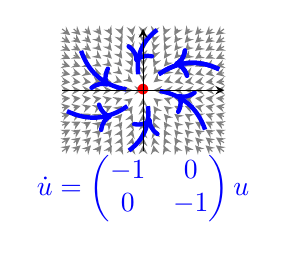
\begin{tikzpicture}
                  \begin{axis}[
                          width=0.3\textwidth,
                          axis lines=middle,
                          no markers,
                          xtick=\empty,
                          ytick=\empty,
                          clip=false,
                          xlabel={},
                          ylabel={},
                          domain=-1:1,
                          ymin=-1, ymax=1,
                          xmin= -1, xmax=1,
                          view = {0}{90}
                      ]

                      \addplot3[gray, quiver={u={-x}, v={-y}, scale arrows=0.1}, -stealth,samples=15] {0};

                      \node[red] (o) at (0, 0) {$\bullet$};

                      \node[blue] at (axis description cs: 0.5, -0.3) {$\dot u = \begin{pmatrix}
                                  -1 & 0  \\
                                  0  & -1
                              \end{pmatrix}u$};

                      \pgfplotsinvokeforeach{0,...,6} {
                          \draw[blue, ultra thick, marking along={0.5}{<}] (o) to[bend left] ({cos(60*#1+20)}, {sin(60*#1+20)});
                      }
                  \end{axis}
              \end{tikzpicture}
              \hspace{1cm}
              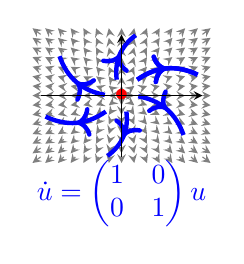
\begin{tikzpicture}
                  \begin{axis}[
                          width=0.3\textwidth,
                          axis lines=middle,
                          no markers,
                          xtick=\empty,
                          ytick=\empty,
                          clip=false,
                          xlabel={},
                          ylabel={},
                          domain=-1:1,
                          ymin=-1, ymax=1,
                          xmin= -1, xmax=1,
                          view = {0}{90}
                      ]

                      \addplot3[gray, quiver={u={x}, v={y}, scale arrows=0.1}, -stealth,samples=15] {0};

                      \node[red] (o) at (0, 0) {$\bullet$};

                      \node[blue] at (axis description cs: 0.5, -0.3) {$\dot u = \begin{pmatrix}
                                  1 & 0 \\
                                  0 & 1
                              \end{pmatrix}u$};

                      \pgfplotsinvokeforeach{0,...,6} {
                          \draw[blue, ultra thick, marking along={0.5}{>}] (o) to[bend left] ({cos(60*#1+20)}, {sin(60*#1+20)});
                      }

                  \end{axis}
              \end{tikzpicture}
              \hspace{1cm}
              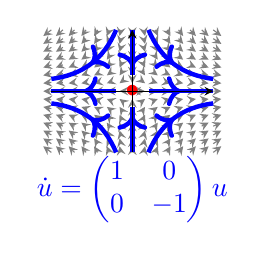
\begin{tikzpicture}
                  \begin{axis}[
                          width=0.3\textwidth,
                          axis lines=middle,
                          no markers,
                          xtick=\empty,
                          ytick=\empty,
                          clip=false,
                          xlabel={},
                          ylabel={},
                          domain=-1:1,
                          ymin=-1, ymax=1,
                          xmin= -1, xmax=1,
                          view = {0}{90}
                      ]

                      \addplot3[gray, quiver={u={x}, v={-y}, scale arrows=0.1}, -stealth,samples=15] {0};

                      \node[red] (o) at (0, 0) {$\bullet$};

                      \node[blue] at (axis description cs: 0.5, -0.3) {$\dot u = \begin{pmatrix}
                                  1 & 0  \\
                                  0 & -1
                              \end{pmatrix}u$};

                      \draw[blue, ultra thick, marking along={0.5}{>}] (o) -- (1, 0);
                      \draw[blue, ultra thick, marking along={0.5}{>}] (o) -- (-1, 0);
                      \draw[blue, ultra thick, marking along={0.5}{<}] (o) -- (0, 1);
                      \draw[blue, ultra thick, marking along={0.5}{<}] (o) -- (0, -1);

                      \draw[blue, ultra thick, marking along={0.5}{>}] (0.2, 1) to[bend right] (1, 0.2);
                      \draw[blue, ultra thick, marking along={0.5}{>}] (-0.2, 1) to[bend left] (-1, 0.2);
                      \draw[blue, ultra thick, marking along={0.5}{>}] (0.2, -1) to[bend left] (1, -0.2);
                      \draw[blue, ultra thick, marking along={0.5}{>}] (-0.2, -1) to[bend right] (-1, -0.2);
                  \end{axis}
              \end{tikzpicture}
          \end{center}

          \color{black}

    \item For each of the two linear systems listed below, classify the equilibrium $u=0$ as attractor, repeller, saddle, or nonhyperbolic depending on the value of $\mu\in\mathbb{R}$:
          \[
              \dot{u} = \begin{pmatrix} -1 & 2 \\ 0 & \mu \end{pmatrix} u, \qquad\qquad
              \dot{u} = \begin{pmatrix} \mu & -1 \\ 1 & \mu \end{pmatrix} u
          \]

          \color{blue}
          \begin{align*}
              \dot{u} = \begin{pmatrix} -1 & 2 \\ 0 & \mu \end{pmatrix} u   & \implies J = \begin{pmatrix} -1 & 2 \\ 0 & \mu \end{pmatrix} \implies \lambda_1 = -1, \lambda_2 = \mu \implies \begin{cases}
                                                                                                                                                                                                 \text{Attractor}     & \text{if } \mu < 0 \\
                                                                                                                                                                                                 \text{Saddle}        & \text{if } \mu > 0 \\
                                                                                                                                                                                                 \text{Nonhyperbolic} & \text{if } \mu = 0
                                                                                                                                                                                             \end{cases}            \\
              \dot{u} = \begin{pmatrix} \mu & -1 \\ 1 & \mu \end{pmatrix} u & \implies J = \begin{pmatrix} \mu & -1 \\ 1 & \mu \end{pmatrix} \implies \lambda_1 = \mu - i, \lambda_2 = \mu + i \implies \begin{cases}
                                                                                                                                                                                                            \text{Attractor}     & \text{if } \mu < 0 \\
                                                                                                                                                                                                            \text{Repeller}      & \text{if } \mu > 0 \\
                                                                                                                                                                                                            \text{Nonhyperbolic} & \text{if } \mu = 0
                                                                                                                                                                                                        \end{cases}
          \end{align*}
          \color{black}
\end{enumerate}

\pagebreak

%%%%%%%%%%%%%%%%%%%%%%%%%%%%%%%%

\section{Competing species model}

We return to our model of two species that compete for food resources. The following system is the same model but I changed some of the values in the equation for the first species:
\begin{eqnarray*}
    \dot{x} & = & x(3-2x-y) \\
    \dot{y} & = & y(2-x-y).
\end{eqnarray*}
Find all equilibria, determine their stability using the eigenvalues of the Jacobian, find and plot the nullclines, and draw a phase portrait that contains representative solutions. Interpret your results in terms of our fictitious two populations.

\color{blue}
Let $f(x, y) = x(3-2x-y)$ and $g(x, y) = y(2-x-y)$. Then, the nullclines of $f$ are given by
\[\left\{(x, y): \; x(3 - 2x- y) = 0\right\} = \{(0, y): y \in \R\} \cup \left\{\left(-\frac{y - 3}{2}, y\right): y \in \R\right\}\]

Similarly, the nullclines of $g$ are given by
\[\left\{(x, y): \; y(2 - x - y) = 0\right\} = \{(x, 0): x \in \R\} \cup \left\{(x, 2-x): x \in \R\right\}\]

\begin{center}
    \color{black}
    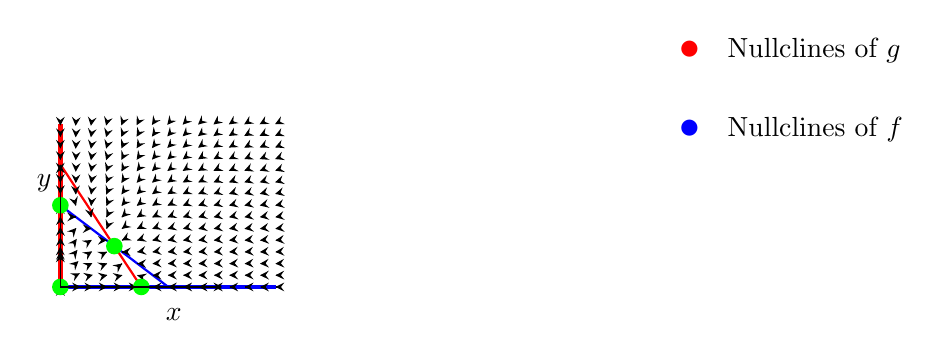
\begin{tikzpicture}
        \begin{axis}[
                width=0.3\textwidth,
                axis lines=middle,
                no markers,
                xtick=\empty,
                ytick=\empty,
                clip=false,
                x label style={at={(axis description cs:0.7, -0.1)},anchor=north},
                y label style={at={(axis description cs:-0.1, 0.7)},anchor=south},
                xlabel={$x$},
                ylabel={$y$},
                domain=0:4,
                ymin=0, ymax=3,
                xmin= 0, xmax=3,
                view = {0}{90}
            ]
            \addplot[name path=b0, blue, ultra thick, domain=0:4] {0};
            \addplot[name path=bd, blue, thick, domain=0:2] {2-x};

            \addplot[name path=r0, red, ultra thick, domain=0:4] ({0}, {x});
            \addplot[name path=rd, red, thick, domain=0:3] ({-x/2 + 3/2}, {x});

            \addplot3[quiver={u={x*(3-2*x-y)/(9*x^2+y^2)}, v={y*(2-x-y)/(9*x^2+y^2)}, scale arrows=0.1}, -stealth,samples=15] {0};

            \fill [name intersections={of=b0 and r0, by={O}}, green] (O) circle (3pt);
            \fill [name intersections={of=bd and rd, by={P}}, green] (P) circle (3pt);
            \fill [name intersections={of=bd and r0, by={R}}, green] (R) circle (3pt);
            \fill [name intersections={of=rd and b0, by={R}}, green] (R) circle (3pt);
        \end{axis}

        \node[scale=1.5, red] (n1) at (8, 3) {$\bullet$};
        \node[scale=1.5, blue] (n2) at (8, 2) {$\bullet$};

        \node[right, xshift=10pt] at (n1) {Nullclines of $g$};
        \node[right, xshift=10pt] at (n2) {Nullclines of $f$};

    \end{tikzpicture}
\end{center}

Immediately, these intersections give us equilibria at $(0, 0)$, $(0, 2)$, $(1, 1)$, and $(3/2, 0)$.

We can take the Jacobian,
\[J(x, y) = \begin{pmatrix}
        3 - 4x - y & -x         \\
        -y         & 2 - x - 2y
    \end{pmatrix}\]
and evaluate:
\begin{align*}
    J(0, 0)   & = \begin{pmatrix}
                      3 & 0 \\
                      0 & 2
                  \end{pmatrix} \implies \lambda = \{3, 2\} \implies \text{repellor}                                                                 \\
    J(0, 2)   & = \begin{pmatrix}
                      1  & 0  \\
                      -2 & -2
                  \end{pmatrix} \implies \lambda = \{1, -2\} \implies \text{saddle}                                                                  \\
    J(1, 1)   & = \begin{pmatrix}
                      -2 & -1 \\
                      -1 & -1
                  \end{pmatrix} \implies \lambda = \{-\frac{3}{2} - \frac{\sqrt 5}{2}, -\frac{3}{2} + \frac{\sqrt 5}{2}\}  \implies \text{attractor} \\
    J(3/2, 0) & = \begin{pmatrix}
                      -3 & -3/2 \\
                      0  & 1/2
                  \end{pmatrix} \implies \lambda = \{-3, 1/2\} \implies \text{saddle}
\end{align*}

So our phase portrait should look something like this:

\begin{center}
    \color{black}
    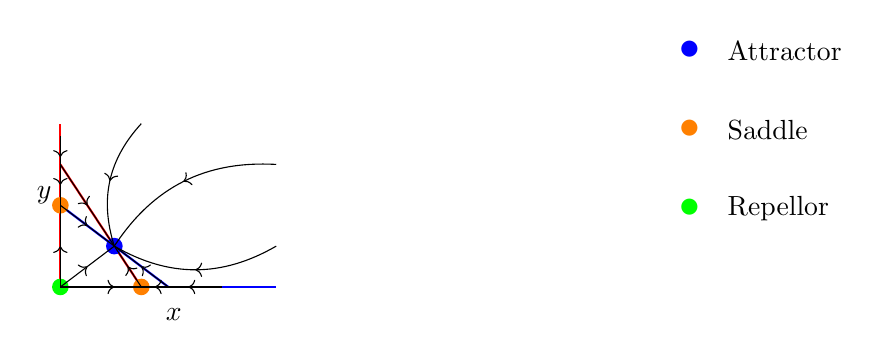
\begin{tikzpicture}
        \begin{axis}[
                width=0.3\textwidth,
                axis lines*=middle,
                no markers,
                xtick=\empty,
                ytick=\empty,
                clip=false,
                x label style={at={(axis description cs:0.7, -0.1)},anchor=north},
                y label style={at={(axis description cs:-0.1, 0.6)},rotate=-90, anchor=south},
                xlabel={$x$},
                ylabel={$y$},
                domain=0:4,
                ymin=0, ymax=3,
                xmin= 0, xmax=3,
                view = {0}{90}
            ]
            \addplot[name path=b0, blue, thick, domain=0:4] {0};
            \addplot[name path=bd, blue, thick, domain=0:2] {2-x};

            \addplot[name path=r0, red, thick, domain=0:4] ({0}, {x});
            \addplot[name path=rd, red, thick, domain=0:3] ({-x/2 + 3/2}, {x});

            \fill [name intersections={of=b0 and r0, by={O}}, green] (O) circle (3pt);
            \fill [name intersections={of=bd and rd, by={11}}, blue] (11) circle (3pt);
            \fill [name intersections={of=bd and b0, by={20}}, red] (20) circle (0pt);
            \fill [name intersections={of=bd and r0, by={02}}, orange] (02) circle (3pt);
            \fill [name intersections={of=rd and r0, by={03}}, red] (03) circle (0pt);
            \fill [name intersections={of=rd and b0, by={320}}, orange] (320) circle (3pt);

            \draw[marking along] (O) -- (11);
            \draw[marking along] (O) -- (20);
            \draw[marking along] (O) -- (02);

            \draw[marking along] (03) -- (11);
            \draw[marking along] (03) -- (02);
            \draw[marking along={0.5}{<}] (03) -- ++(0, 0.7);

            \draw[marking along] (02) -- (11);

            \draw[marking along] (20) -- (11);
            \draw[marking along] (20) -- (320);
            \draw[marking along={0.5}{<}] (20) -- ++(1, 0);

            \draw[marking along] (320) -- (11);

            \draw[marking along] (1.5, 4) to[bend right] (11);
            \draw[marking along] (4, 3) to[bend right] (11);

            \draw[marking along] (4, 1) to[bend left] (11);
        \end{axis}

        \node[scale=1.5, blue] (n2) at (8, 3) {$\bullet$};
        \node[scale=1.5, orange] (n3) at (8, 2) {$\bullet$};
        \node[scale=1.5, green] (n4) at (8, 1) {$\bullet$};


        \node[right, xshift=10pt] at (n2) {Attractor};
        \node[right, xshift=10pt] at (n3) {Saddle};
        \node[right, xshift=10pt] at (n4) {Repellor};
    \end{tikzpicture}
\end{center}

When we first saw this model in class, we had two competing species with no possible stable coexistence. Here, however, we can see that it is possible for a species to die out or for the two species to coexist at the equilibrium.
\color{black}

\end{document}